% LaTeX 2e Document.
% 
% $Id: sort.vdm,v 1.11 2005/05/13 00:41:46 vdmtools Exp $
% 

%%%%%%%%%%%%%%%%%%%%%%%%%%%%%%%%%%%%%%%%
% PDF compatibility code. 
\makeatletter
\newif\ifpdflatex@
\ifx\pdftexversion\@undefined
\pdflatex@false
%\message{Not using pdf}
\else
\pdflatex@true
%\message{Using pdf}
\fi

\newcommand{\latexorpdf}[2]{
  \ifpdflatex@ #2
  \else #1
  \fi
}

\newcommand{\pformat}{a4paper}

\makeatother
%%%%%%%%%%%%%%%%%%%%%%%%%%%%%%%%%%%%%%%%

\latexorpdf{
\documentclass[\pformat,12pt]{article}
}{
\documentclass[\pformat,pdftex,12pt]{article}
}

\usepackage{color}
\usepackage{vdmsl-2e}
\usepackage{vpp}
\usepackage{longtable}
\usepackage{alltt}
\usepackage{makeidx}
\usepackage{graphics}
% graphics includes
\usepackage{graphicx}

\newcommand{\StateDef}[1]{{\bf #1}}
\newcommand{\TypeDef}[1]{{\bf #1}}
\newcommand{\TypeOcc}[1]{{\it #1}}
\newcommand{\FuncDef}[1]{{\bf #1}}
\newcommand{\FuncOcc}[1]{{#1}}
\newcommand{\ModDef}[1]{{\tiny #1}}
\newcommand{\MethodDef}[1]{{\bf #1}}
\newcommand{\MethodOcc}[1]{{#1}}

\definecolor{covered}{rgb}{0,0,0}      %black
\definecolor{not-covered}{rgb}{1,0,0}   %gray for previewing
%\definecolor{not_covered}{gray}{0.6}   %gray for printing
\definecolor{not_covered}{rgb}{1,0,0}  %red

\title{The Concurrent Missile VDM++ Model}
\author{Peter Gorm Larsen and Marcel Verhoef}
\date{2007}

\makeindex

\begin{document}
\maketitle

\section{The Overall Class Diagram}

\begin{figure}[h]
\begin{center}
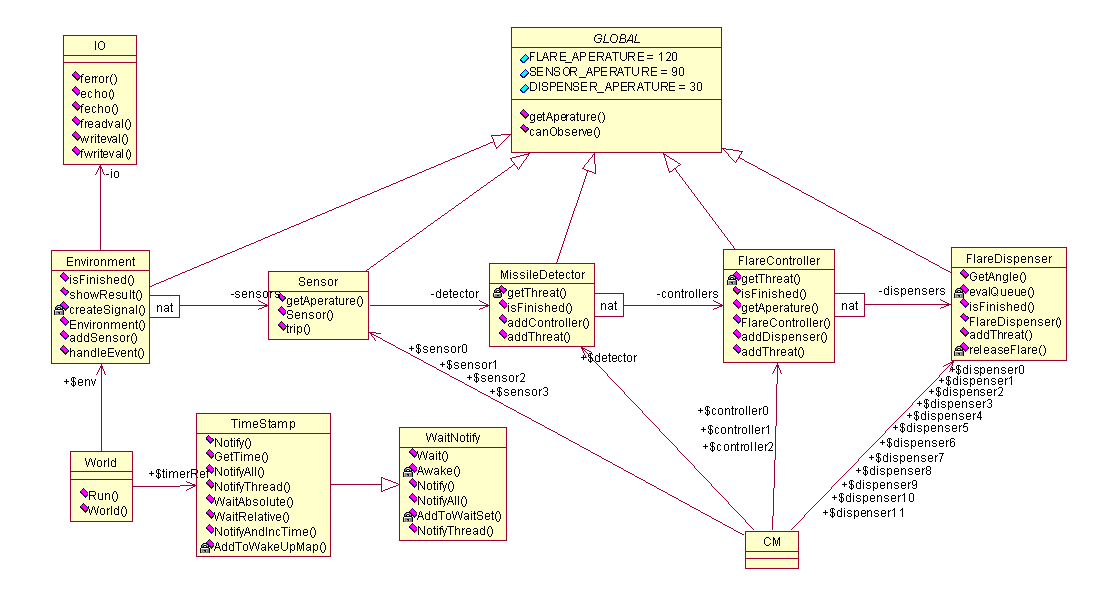
\includegraphics[width=\textwidth]{concurCMclassdiag.png}
\end{center}
\caption{Overview of the classes in the concurrent CM model}\label{fig:inputoutput}
\end{figure}
\newpage

\section{The World Class}

\begin{vdm}{\small\sf class} $World$\index{World|ModDef}
\par
\kInstanceVarDef
\parlinebr
\begin{insvar}
\assdef{sensor}{Sensor\index{Sensor|TypeOcc}}[{\fnapply{\new{Sensor}}{}}]
\end{insvar}
\begin{insvar}
\assdef{detector}{MissileDetector\index{MissileDetector|TypeOcc}}[{\fnapply{\new{MissileDetector}}{}}]
\end{insvar}
\begin{insvar}
\assdef{flareControl}{FlareController\index{FlareController|TypeOcc}}[{\fnapply{\new{FlareController}}{}}]
\end{insvar}
\begin{insvar}
\assdef{timerRef}{Timer\index{Timer|TypeOcc}}[{\fnapply{\new{Timer}}{}}]
\end{insvar}
\par
\kOperations
\kw{\kw{public}}\begin{op}[e]{Run}\index{Run|FuncDef}%
\signature{() \Oto FlareDispenser`MagId\index{MagId|TypeOcc} \Gmap \seqof*{\Lp FlareDispenser`FlareType\index{FlareType|TypeOcc} \X \Nat  \Rp }}
\parms{}
\annlab[o]{World`Run}
\begin{blockstmt}
$sensor$.\call{Init}{timerRef} ; \\
$detector$.\call{Init}{sensor,flareControl} ; \\
$flareControl$.\call{Init}{detector,timerRef} ; \\

\start{sensor} ; \\

\start{detector} ; \\

\start{flareControl} ; \\
$sensor$.\call{IsFinished}{} ; \\
$detector$.\call{IsFinished}{} ; \\
\return{\fnapply{flareControl.IsFinished}{}}
\end{blockstmt}
\end{op}
{\small\sf end} {\it World}

\end{vdm}




























\begin{tabular}{p{25mm}l}
{\bf Test Suite :} & vdm.tc \\ 
{\bf Class :} & World \\ 
\end{tabular}

\begin{longtable}{|l|r|r|}\hline
{\bf World`Run} & {\bf \#Calls} & {\bf Coverage} \kill
{\bf Name} & {\bf \#Calls} & {\bf Coverage} \\ \hline\hline
\endhead
World`Run & 1 & $\surd$ \\ \hline
\hline
{\bf Total Coverage} & & {\bf 100\%} \\ \hline
\end{longtable}




\section{The FighterAircraft Class}

\begin{vdm}{\small\sf class} $FighterAircraft$\index{FighterAircraft|ModDef}
\par
\kInstanceVarDef
\parlinebr
\begin{insvar}\kw{public}\kw{ }\kw{static}
\assdef{detector}{MissileDetector\index{MissileDetector|TypeOcc}}[{\fnapply{\new{MissileDetector}}{}}]
\end{insvar}
\begin{insvar}\kw{public}\kw{ }\kw{static}
\assdef{sensor0}{Sensor\index{Sensor|TypeOcc}}[{\fnapply{\new{Sensor}}{detector,0}}]
\end{insvar}
\begin{insvar}\kw{public}\kw{ }\kw{static}
\assdef{sensor1}{Sensor\index{Sensor|TypeOcc}}[{\fnapply{\new{Sensor}}{detector,90}}]
\end{insvar}
\begin{insvar}\kw{public}\kw{ }\kw{static}
\assdef{sensor2}{Sensor\index{Sensor|TypeOcc}}[{\fnapply{\new{Sensor}}{detector,180}}]
\end{insvar}
\begin{insvar}\kw{public}\kw{ }\kw{static}
\assdef{sensor3}{Sensor\index{Sensor|TypeOcc}}[{\fnapply{\new{Sensor}}{detector,270}}]
\end{insvar}
\begin{insvar}\kw{public}\kw{ }\kw{static}
\assdef{controller0}{FlareController\index{FlareController|TypeOcc}}[{\fnapply{\new{FlareController}}{0}}]
\end{insvar}
\begin{insvar}\kw{public}\kw{ }\kw{static}
\assdef{controller1}{FlareController\index{FlareController|TypeOcc}}[{\fnapply{\new{FlareController}}{120}}]
\end{insvar}
\begin{insvar}\kw{public}\kw{ }\kw{static}
\assdef{controller2}{FlareController\index{FlareController|TypeOcc}}[{\fnapply{\new{FlareController}}{240}}]
\end{insvar}
\begin{insvar}\kw{public}\kw{ }\kw{static}
\assdef{dispenser0}{FlareDispenser\index{FlareDispenser|TypeOcc}}[{\fnapply{\new{FlareDispenser}}{0}}]
\end{insvar}
\begin{insvar}\kw{public}\kw{ }\kw{static}
\assdef{dispenser1}{FlareDispenser\index{FlareDispenser|TypeOcc}}[{\fnapply{\new{FlareDispenser}}{30}}]
\end{insvar}
\begin{insvar}\kw{public}\kw{ }\kw{static}
\assdef{dispenser2}{FlareDispenser\index{FlareDispenser|TypeOcc}}[{\fnapply{\new{FlareDispenser}}{60}}]
\end{insvar}
\begin{insvar}\kw{public}\kw{ }\kw{static}
\assdef{dispenser3}{FlareDispenser\index{FlareDispenser|TypeOcc}}[{\fnapply{\new{FlareDispenser}}{90}}]
\end{insvar}
\begin{insvar}\kw{public}\kw{ }\kw{static}
\assdef{dispenser4}{FlareDispenser\index{FlareDispenser|TypeOcc}}[{\fnapply{\new{FlareDispenser}}{0}}]
\end{insvar}
\begin{insvar}\kw{public}\kw{ }\kw{static}
\assdef{dispenser5}{FlareDispenser\index{FlareDispenser|TypeOcc}}[{\fnapply{\new{FlareDispenser}}{30}}]
\end{insvar}
\begin{insvar}\kw{public}\kw{ }\kw{static}
\assdef{dispenser6}{FlareDispenser\index{FlareDispenser|TypeOcc}}[{\fnapply{\new{FlareDispenser}}{60}}]
\end{insvar}
\begin{insvar}\kw{public}\kw{ }\kw{static}
\assdef{dispenser7}{FlareDispenser\index{FlareDispenser|TypeOcc}}[{\fnapply{\new{FlareDispenser}}{90}}]
\end{insvar}
\begin{insvar}\kw{public}\kw{ }\kw{static}
\assdef{dispenser8}{FlareDispenser\index{FlareDispenser|TypeOcc}}[{\fnapply{\new{FlareDispenser}}{0}}]
\end{insvar}
\begin{insvar}\kw{public}\kw{ }\kw{static}
\assdef{dispenser9}{FlareDispenser\index{FlareDispenser|TypeOcc}}[{\fnapply{\new{FlareDispenser}}{30}}]
\end{insvar}
\begin{insvar}\kw{public}\kw{ }\kw{static}
\assdef{dispenser10}{FlareDispenser\index{FlareDispenser|TypeOcc}}[{\fnapply{\new{FlareDispenser}}{60}}]
\end{insvar}
\begin{insvar}\kw{public}\kw{ }\kw{static}
\assdef{dispenser11}{FlareDispenser\index{FlareDispenser|TypeOcc}}[{\fnapply{\new{FlareDispenser}}{90}}]
\end{insvar}
\par
{\small\sf end} {\it FighterAircraft}

\end{vdm}




































\section{The Environment Class}

\begin{vdm}{\small\sf class} $Environment$ {\small\sf is subclass of}  $GLOBAL$\index{Environment|ModDef}
\par
\kTypes
\type{\kw{public}\kw{ }inline\index{inline|TypeDef}}{EventId\index{EventId|TypeOcc} \X MissileType\index{MissileType|TypeOcc} \X Angle\index{Angle|TypeOcc} \X \Nat ;}
\type{\kw{public}\kw{ }outline\index{outline|TypeDef}}{EventId\index{EventId|TypeOcc} \X FlareType\index{FlareType|TypeOcc} \X Angle\index{Angle|TypeOcc} \X \Nat  \X \Nat }
\kInstanceVarDef
\parlinebr
\begin{insvar}
\assdef{io}{IO\index{IO|TypeOcc}}[{\fnapply{\new{IO}}{}}]
\end{insvar}
\begin{insvar}
\assdef{inlines}{\seqof*{inline\index{inline|TypeOcc}}}[{\seq{}}]
\end{insvar}
\begin{insvar}
\assdef{busy}{\Bool }[{\True }]
\end{insvar}
\begin{insvar}
\assdef{outlines}{\seqof*{outline\index{outline|TypeOcc}}}[{\seq{}}]
\end{insvar}
\begin{insvar}
\assdef{ranges}{\Nat  \Gmap \Lp Angle\index{Angle|TypeOcc} \X Angle\index{Angle|TypeOcc} \Rp }[{\Emptymap }]
\end{insvar}
\begin{insvar}
\assdef{sensors}{\Nat  \Gmap Sensor\index{Sensor|TypeOcc}}[{\Emptymap }]
\end{insvar}
\begin{instinvfn}
 \Dom ranges =  \Dom sensors\end{instinvfn}
\begin{insvar}
\assdef{evid}{\Opt{EventId\index{EventId|TypeOcc}}}[{\Nil }]
\end{insvar}
\par
\kOperations
\kw{\kw{public}}\begin{op}[e]{Environment}\index{Environment|FuncDef}%
\signature{\seqof*{\Char } \Oto Environment\index{Environment|TypeOcc}}
\parms{fname}
\annlab[o]{Environment`Environment}
\begin{defstmt}
\eqdef{\reccons{\kw{mk-}}{-,input}}{\fnapply{io.freadval[\seqof*{inline\index{inline|TypeOcc}}]}{fname}}
\end{defstmt} \\
\ass{inlines}{input};
\end{op}
\kw{\kw{public}}\begin{op}[e]{addSensor}\index{addSensor|FuncDef}%
\signature{Sensor\index{Sensor|TypeOcc} \Oto ()}
\parms{psens}
\annlab[o]{Environment`addSensor}
\begin{blockstmt}
\begin{dclstmt}
\assdef{id}{\Nat }[{ \Card  \Dom ranges + 1}]
\end{dclstmt}
\kw{atomic }
\begin{blockstmt}\color{not-covered}\ass{ranges}{ranges \Mapmerge \map{id \Mapsto \fnapply{psens.getAperature}{}}}\color{covered} ; \\
\color{not-covered}\ass{sensors}{sensors \Mapmerge \map{id \Mapsto psens}}\color{covered}
\end{blockstmt}
\end{blockstmt};
\end{op}
\kw{\kw{private}}\begin{op}[e]{createSignal}\index{createSignal|FuncDef}%
\signature{() \Oto \Opt{EventId\index{EventId|TypeOcc}}}
\parms{}
\annlab[o]{Environment`createSignal}
\begin{blockstmt}
\If  \Len inlines > 0
\Then \\
\begin{blockstmt}
\begin{dclstmt}
\assdef{curtime}{\Nat }[{\fnapply{World`timerRef.GetTime}{}}]
\assdef{done}{\Bool }[{\False }]
\end{dclstmt}
\begin{while}{ \Not done}
\begin{defstmt}
\eqdef{\reccons{\kw{mk-}}{eventid,pmt,pa,pt}}{ \Hd inlines}
\end{defstmt} \\
\If pt \Le curtime
\Then \\
\begin{blockstmt}
\begin{setfor}{id}{ \Dom ranges}
\begin{defstmt}
\eqdef{\reccons{\kw{mk-}}{papplhs,pappsize}}{\fnapply{ranges}{id}}
\end{defstmt} \\
\If \fnapply{canObserve}{pa,papplhs,pappsize}
\Then \\
\fnapply{sensors}{id}.\call{trip}{eventid,pmt,pa}
\Fi
\end{setfor} ; \\
\ass{inlines}{ \Tl inlines} ; \\
\ass{done}{ \Len inlines = 0} ; \\
\return{eventid}
\end{blockstmt}
\Else \\
\begin{blockstmt}
\ass{done}{\True } ; \\
\return{\Nil }
\end{blockstmt}
\Fi
\end{while}
\end{blockstmt}
\Else \\
\begin{blockstmt}
\ass{busy}{\False } ; \\
\return{\Nil }
\end{blockstmt}
\Fi
\end{blockstmt};
\end{op}
\kw{\kw{public}}\begin{op}[e]{handleEvent}\index{handleEvent|FuncDef}%
\signature{EventId\index{EventId|TypeOcc} \X FlareType\index{FlareType|TypeOcc} \X Angle\index{Angle|TypeOcc} \X \Nat  \X \Nat  \Oto ()}
\parms{evid,pfltp,angle,pt1,pt2}
\annlab[o]{Environment`handleEvent}
\begin{blockstmt}
\ass{outlines}{outlines \Sconc \seq{\reccons{\kw{mk-}}{evid,pfltp,angle,pt1,pt2}}}
\end{blockstmt};
\end{op}
\kw{\kw{public}}\begin{op}[e]{showResult}\index{showResult|FuncDef}%
\signature{() \Oto ()}
\parms{}
\annlab[o]{Environment`showResult}
\begin{defstmt}
\eqdef{-}{\fnapply{io.writeval[\seqof*{outline\index{outline|TypeOcc}}]}{outlines}}
\end{defstmt} \\
\Skip ;
\end{op}
\kw{\kw{public}}\begin{op}[e]{isFinished}\index{isFinished|FuncDef}%
\signature{() \Oto ()}
\parms{}
\annlab[o]{Environment`isFinished}
\Skip 
\end{op}
\kSync

\mutex{handleEvent};

\index{isFinished|MethodOcc}
\per{isFinished}{
 \Not busy
}

\kThreadDef
\begin{thread}
\begin{while}{\True }
\begin{blockstmt}
\If busy
\Then \\
\begin{blockstmt}
\ass{evid}{\fnapply{createSignal}{}}
\end{blockstmt}
\Fi ; \\
World`timerRef.\call{NotifyAndIncTime}{}
\end{blockstmt}
\end{while}
\end{thread}
{\small\sf end} {\it Environment}

\end{vdm}























































































\begin{tabular}{p{25mm}l}
{\bf Test Suite :} & vdm.tc \\ 
{\bf Class :} & Environment \\ 
\end{tabular}

\begin{longtable}{|l|r|r|}\hline
{\bf Environment`createSignal} & {\bf \#Calls} & {\bf Coverage} \kill
{\bf Name} & {\bf \#Calls} & {\bf Coverage} \\ \hline\hline
\endhead
Environment`addSensor & 4 & $\surd$ \\ \hline
Environment`isFinished & 1 & $\surd$ \\ \hline
Environment`showResult & 1 & $\surd$ \\ \hline
Environment`Environment & 1 & $\surd$ \\ \hline
Environment`handleEvent & 21 & $\surd$ \\ \hline
Environment`createSignal & 82 & $\surd$ \\ \hline
\hline
{\bf Total Coverage} & & {\bf 100\%} \\ \hline
\end{longtable}





\section{The Global Class}

\begin{vdm}{\small\sf class} $GLOBAL$\index{GLOBAL|ModDef}
\par
\kValues
\kw{\kw{public}}\val{SENSOR-APERATURE}{90;}
\kw{\kw{public}}\val{FLARE-APERATURE}{120;}
\kw{\kw{public}}\val{DISPENSER-APERATURE}{30}
\kTypes
\type{\kw{public}\kw{ }MissileType\index{MissileType|TypeDef}}{\const{MissileA} | \const{MissileB} | \const{MissileC} | \const{None};}
\type{\kw{public}\kw{ }FlareType\index{FlareType|TypeDef}}{\const{FlareOneA} | \const{FlareTwoA} | \const{DoNothingA} |  \\
\const{FlareOneB} | \const{FlareTwoB} | \const{DoNothingB} |  \\
\const{FlareOneC} | \const{FlareTwoC} | \const{DoNothingC};}
\type{\kw{public}\kw{ }Angle\index{Angle|TypeDef}}{\Nat }
\begin{invfn}{num}num < 360;
\end{invfn}
\type{\kw{public}\kw{ }EventId\index{EventId|TypeDef}}{\Nat }
\kOperations
\kw{\kw{public}}\begin{op}[e]{canObserve}\index{canObserve|FuncDef}%
\signature{Angle\index{Angle|TypeOcc} \X Angle\index{Angle|TypeOcc} \X Angle\index{Angle|TypeOcc} \Oto \Bool }
\parms{pangle,pleft,psize}
\annlab[o]{GLOBAL`canObserve}
\begin{defstmt}
\eqdef{pright}{\pex{pleft + psize} \Mod 360}
\end{defstmt} \\
\If pright < pleft
\Then \\
\return{\pex{pangle < pright \Or pangle \Ge pleft}}
\Else \\
\return{\pex{pangle \Ge pleft \And pangle < pright}}
\Fi;
\end{op}
\kw{\kw{public}}\begin{op}[e]{getAperature}\index{getAperature|FuncDef}%
\signature{() \Oto Angle\index{Angle|TypeOcc} \X Angle\index{Angle|TypeOcc}}
\parms{}
\annlab[o]{GLOBAL`getAperature}
\issubclassresp
\end{op}
{\small\sf end} {\it GLOBAL}

\end{vdm}







































\begin{tabular}{p{25mm}l}
{\bf Test Suite :} & vdm.tc \\ 
{\bf Class :} & GLOBAL \\ 
\end{tabular}

\begin{longtable}{|l|r|r|}\hline
{\bf GLOBAL`canObserve} & {\bf \#Calls} & {\bf Coverage} \kill
{\bf Name} & {\bf \#Calls} & {\bf Coverage} \\ \hline\hline
\endhead
GLOBAL`canObserve & 84 & $\surd$ \\ \hline
GLOBAL`getAperature & 0 & 0\% \\ \hline
\hline
{\bf Total Coverage} & & {\bf 96\%} \\ \hline
\end{longtable}




\section{The Sensor Class}

\begin{vdm}{\small\sf class} $Sensor$\index{Sensor|ModDef}
\par
\kTypes
\type{\kw{public}\kw{ }MissileType\index{MissileType|TypeDef}}{\const{MissileA} | \const{MissileB} | \const{MissileC} | \const{None};}
\type{\kw{public}\kw{ }Angle\index{Angle|TypeDef}}{\Nat }
\begin{invfn}{num}num \Le 360
\end{invfn}
\kInstanceVarDef
\parlinebr
\begin{insvar}
\assdef{io}{SensorIO\index{SensorIO|TypeOcc}}[{\fnapply{\new{SensorIO}}{}}]
\end{insvar}
\begin{insvar}
\assdef{threat}{\Opt{\Lp MissileType\index{MissileType|TypeOcc} | \const{Consumed} \Rp  \X Angle\index{Angle|TypeOcc}}}[{\fnapply{io.readThreat}{}}]
\end{insvar}
\begin{insvar}
\assdef{timerRef}{Timer\index{Timer|TypeOcc}}
\end{insvar}
\par
\kThreadDef
\begin{thread}
\begin{blockstmt}
\begin{while}{threat \Neq \Nil }
\begin{blockstmt}
\call{ThreatConsumed}{} ; \\
\call{SetThreat}{} ; \\
$timerRef$.\call{StepTime}{}
\end{blockstmt}
\end{while} ; \\
$timerRef$.\call{Finished}{}
\end{blockstmt}
\end{thread}
\kOperations
\begin{op}[e]{ThreatConsumed}\index{ThreatConsumed|FuncDef}%
\signature{() \Oto ()}
\parms{}
\annlab[o]{Sensor`ThreatConsumed}
\Skip 
\end{op}
\kSync
\index{ThreatConsumed|MethodOcc}
\per{ThreatConsumed}{
threat \Neq \Nil  \And threat.\#1 = \const{Consumed}
}

\kOperations
\kw{\kw{public}}\begin{op}[e]{Init}\index{Init|FuncDef}%
\signature{Timer\index{Timer|TypeOcc} \Oto ()}
\parms{newTimer}
\annlab[o]{Sensor`Init}
\ass{timerRef}{newTimer};
\end{op}
\begin{op}[e]{SetThreat}\index{SetThreat|FuncDef}%
\signature{() \Oto ()}
\parms{}
\annlab[o]{Sensor`SetThreat}
\ass{threat}{\fnapply{io.readThreat}{}}
\end{op}
\kSync

\mutex{SetThreat,GetThreat}

\kOperations
\kw{\kw{public}}\begin{op}[e]{IsFinished}\index{IsFinished|FuncDef}%
\signature{() \Oto ()}
\parms{}
\annlab[o]{Sensor`IsFinished}
\Skip 
\end{op}
\kSync
\index{IsFinished|MethodOcc}
\per{IsFinished}{
threat = \Nil 
}

\kOperations
\kw{\kw{public}}\begin{op}[e]{GetThreat}\index{GetThreat|FuncDef}%
\signature{() \Oto \Opt{MissileType\index{MissileType|TypeOcc} \X Angle\index{Angle|TypeOcc}}}
\parms{}
\annlab[o]{Sensor`GetThreat}
\begin{letstmt}
\patdef{orgThreat}{threat}
\end{letstmt} \\
\begin{blockstmt}
\If threat \Neq \Nil 
\Then \\
\ass{threat}{\reccons{\kw{mk-}}{\const{Consumed},0}}
\Fi ; \\
\return{orgThreat}
\end{blockstmt}
\end{op}
\kSync
\index{GetThreat|MethodOcc}
\per{GetThreat}{
threat \Neq \Nil  \Implies threat.\#1 \Neq \const{Consumed}
}

{\small\sf end} {\it Sensor}

\end{vdm}









































































\begin{tabular}{p{25mm}l}
{\bf Test Suite :} & vdm.tc \\ 
{\bf Class :} & Sensor \\ 
\end{tabular}

\begin{longtable}{|l|r|r|}\hline
{\bf Sensor`ThreatConsumed} & {\bf \#Calls} & {\bf Coverage} \kill
{\bf Name} & {\bf \#Calls} & {\bf Coverage} \\ \hline\hline
\endhead
Sensor`Init & 1 & $\surd$ \\ \hline
Sensor`GetThreat & 9 & $\surd$ \\ \hline
Sensor`SetThreat & 8 & $\surd$ \\ \hline
Sensor`IsFinished & 1 & $\surd$ \\ \hline
Sensor`ThreatConsumed & 8 & $\surd$ \\ \hline
\hline
{\bf Total Coverage} & & {\bf 100\%} \\ \hline
\end{longtable}




\section{The Missile Detector Class}

\begin{vdm}{\small\sf class} $MissileDetector$ {\small\sf is subclass of}  $GLOBAL$\index{MissileDetector|ModDef}
\par
\kInstanceVarDef
\parlinebr
\begin{insvar}
\assdef{ranges}{\Nat  \Gmap \Lp Angle\index{Angle|TypeOcc} \X Angle\index{Angle|TypeOcc} \Rp }[{\Emptymap }]
\end{insvar}
\begin{insvar}
\assdef{controllers}{\Nat  \Gmap FlareController\index{FlareController|TypeOcc}}[{\Emptymap }]
\end{insvar}
\begin{instinvfn}
 \Dom ranges =  \Dom controllers\end{instinvfn}
\begin{insvar}
\assdef{threats}{\seqof*{\Lp EventId\index{EventId|TypeOcc} \X MissileType\index{MissileType|TypeOcc} \X Angle\index{Angle|TypeOcc} \X \Nat  \Rp }}[{\seq{}}]
\end{insvar}
\begin{insvar}
\assdef{busy}{\Bool }[{\False }]
\end{insvar}
\par
\kOperations
\kw{\kw{public}}\begin{op}[e]{addController}\index{addController|FuncDef}%
\signature{FlareController\index{FlareController|TypeOcc} \Oto ()}
\parms{pctrl}
\annlab[o]{MissileDetector`addController}
\begin{blockstmt}
\begin{dclstmt}
\assdef{nid}{\Nat }[{ \Card  \Dom ranges + 1}]
\end{dclstmt}
\kw{atomic }
\begin{blockstmt}\color{not-covered}\ass{ranges}{ranges \Mapmerge \map{nid \Mapsto \fnapply{pctrl.getAperature}{}}}\color{covered} ; \\
\color{not-covered}\ass{controllers}{controllers \Mapmerge \map{nid \Mapsto pctrl}}\color{covered}
\end{blockstmt} ; \\

\start{pctrl}
\end{blockstmt};
\end{op}
\kw{\kw{public}}\begin{op}[e]{addThreat}\index{addThreat|FuncDef}%
\signature{EventId\index{EventId|TypeOcc} \X MissileType\index{MissileType|TypeOcc} \X Angle\index{Angle|TypeOcc} \X \Nat  \Oto ()}
\parms{evid,pmt,pa,pt}
\annlab[o]{MissileDetector`addThreat}
\begin{blockstmt}
\ass{threats}{threats \Sconc \seq{\reccons{\kw{mk-}}{evid,pmt,pa,pt}}} ; \\
\ass{busy}{\True }
\end{blockstmt};
\end{op}
\kw{\kw{private}}\begin{op}[e]{getThreat}\index{getThreat|FuncDef}%
\signature{() \Oto EventId\index{EventId|TypeOcc} \X MissileType\index{MissileType|TypeOcc} \X Angle\index{Angle|TypeOcc} \X \Nat }
\parms{}
\annlab[o]{MissileDetector`getThreat}
\begin{blockstmt}
\begin{dclstmt}
\assdef{res}{EventId\index{EventId|TypeOcc} \X MissileType\index{MissileType|TypeOcc} \X Angle\index{Angle|TypeOcc} \X \Nat }[{ \Hd threats}]
\end{dclstmt}
\ass{threats}{ \Tl threats} ; \\
\return{res}
\end{blockstmt};
\end{op}
\kw{\kw{public}}\begin{op}[e]{isFinished}\index{isFinished|FuncDef}%
\signature{() \Oto ()}
\parms{}
\annlab[o]{MissileDetector`isFinished}
\begin{setfor}{id}{ \Dom controllers}
\fnapply{controllers}{id}.\call{isFinished}{}
\end{setfor}
\end{op}
\kSync

\mutex{addThreat,getThreat};

\index{getThreat|MethodOcc}
\per{getThreat}{
 \Len threats > 0
};

\index{isFinished|MethodOcc}
\per{isFinished}{
 \Not busy
}

\kThreadDef
\begin{thread}
\begin{while}{\True }
\begin{blockstmt}
\begin{defstmt}
\eqdef{\reccons{\kw{mk-}}{evid,pmt,pa,pt}}{\fnapply{getThreat}{}}
\end{defstmt} \\
\begin{setfor}{id}{ \Dom ranges}
\begin{defstmt}
\eqdef{\reccons{\kw{mk-}}{papplhs,pappsize}}{\fnapply{ranges}{id}}
\end{defstmt} \\
\If \fnapply{canObserve}{pa,papplhs,pappsize}
\Then \\
\fnapply{controllers}{id}.\call{addThreat}{evid,pmt,pa,pt}
\Fi
\end{setfor} ; \\
\ass{busy}{ \Len threats > 0}
\end{blockstmt}
\end{while}
\end{thread}
{\small\sf end} {\it MissileDetector}

\end{vdm}










































































\begin{tabular}{p{25mm}l}
{\bf Test Suite :} & vdm.tc \\ 
{\bf Class :} & MissileDetector \\ 
\end{tabular}

\begin{longtable}{|l|r|r|}\hline
{\bf MissileDetector`addController} & {\bf \#Calls} & {\bf Coverage} \kill
{\bf Name} & {\bf \#Calls} & {\bf Coverage} \\ \hline\hline
\endhead
MissileDetector`addThreat & 7 & $\surd$ \\ \hline
MissileDetector`getThreat & 7 & $\surd$ \\ \hline
MissileDetector`isFinished & 1 & $\surd$ \\ \hline
MissileDetector`addController & 3 & $\surd$ \\ \hline
\hline
{\bf Total Coverage} & & {\bf 100\%} \\ \hline
\end{longtable}




\section{The Flare Controller Class}

\begin{vdm}{\small\sf class} $FlareController$
\par
\kInstanceVarDef
\parlinebr
\begin{insvar}
\assdef{dispensers}{FlareDispenser`MagId \Gmap FlareDispenser}
\end{insvar}
\begin{insvar}
\assdef{missileDetectorRef}{MissileDetector}
\end{insvar}
\begin{insvar}
\assdef{noMoreMissiles}{\Bool }[{\False }]
\end{insvar}
\par
\kValues
\val{mag1}[FlareDispenser`MagId]{\color{not-covered}\reccons{\kw{mk-} \Token}{\Dquote Magazine\hspace{0.5em}1 \Dquote }\color{covered};}
\val{mag2}[FlareDispenser`MagId]{\color{not-covered}\reccons{\kw{mk-} \Token}{\Dquote Magazine\hspace{0.5em}2 \Dquote }\color{covered};}
\val{mag3}[FlareDispenser`MagId]{\color{not-covered}\reccons{\kw{mk-} \Token}{\Dquote Magazine\hspace{0.5em}3 \Dquote }\color{covered};}
\val{mag4}[FlareDispenser`MagId]{\color{not-covered}\reccons{\kw{mk-} \Token}{\Dquote Magazine\hspace{0.5em}4 \Dquote }\color{covered};}
\val{magids}[\setof{FlareDispenser`MagId}]{\color{not-covered}\set{mag1,mag2,mag3,mag4}\color{covered}}
\kOperations
\kw{\kw{public}}\begin{op}[e]{Init}%
\signature{MissileDetector \X Timer \Oto ()}
\parms{initMissileDetector,initTimerRef}
\annlab[o]{FlareController`Init}
\begin{blockstmt}
\ass{missileDetectorRef}{initMissileDetector} ; \\
\ass{dispensers}{\mapcomp{mag \Mapsto \fnapply{\new{FlareDispenser}}{mag,initTimerRef}} \\
{mag \In magids}}
\end{blockstmt};
\end{op}
\kw{\kw{public}}\begin{op}[e]{Step}%
\signature{() \Oto ()}
\parms{}
\annlab[o]{FlareController`Step}
\begin{setfor}{magid}{magids}
\fnapply{dispensers}{magid}.\call{Step}{}
\end{setfor};
\end{op}
\kw{\kw{public}}\begin{op}[e]{IsFinished}%
\signature{() \Oto \Bool }
\parms{}
\annlab[o]{FlareController`IsFinished}
\return{noMoreMissiles \And  \\
\all{magid \In magids}{\fnapply{\fnapply{dispensers}{magid}.GetCurrentStep}{} = 0}};
\end{op}
\kw{\kw{public}}\begin{op}[e]{GetResult}%
\signature{() \Oto FlareDispenser`MagId \Gmap \seqof*{\Lp FlareDispenser`FlareType \X \Nat  \Rp }}
\parms{}
\annlab[o]{FlareController`GetResult}
\return{\mapcomp{magid \Mapsto \fnapply{\fnapply{dispensers}{magid}.GetResult}{}}{magid \In magids}};
\end{op}
\kw{\kw{public}}\begin{op}[e]{MissileIsHere}%
\signature{\Opt{Sensor`MissileType \X Sensor`Angle} \Oto ()}
\parms{newMissileValue}
\annlab[o]{FlareController`MissileIsHere}
\begin{blockstmt}
\If newMissileValue = \Nil 
\Then \\
\ass{noMoreMissiles}{\True }
\Elseif newMissileValue.\#1 \Neq \const{None}
\Then \\
\begin{letstmt}
\patdef{\reccons{\kw{mk-}}{misType,angle}}{newMissileValue}
\patdef{magid}{\fnapply{Angle2MagId}{angle}}
\end{letstmt} \\
\fnapply{dispensers}{magid}.\call{NewMissileValue}{misType}
\Fi
\end{blockstmt}
\end{op}
\kFunctions
\begin{fn}[e]{Angle2MagId}%
\signature{Sensor`Angle \To FlareDispenser`MagId}
\parms*{\Lp angle\Rp }
\annlab[o]{FlareController`Angle2MagId}
\If angle < 90
\Then \\
mag1
\Elseif angle < 180
\Then \\
mag2
\Elseif angle < 270
\Then \\
mag3
\Else \\
mag4
\Fi
\end{fn}
{\small\sf end} {\it FlareController}

\end{vdm}



































































\begin{tabular}{p{25mm}l}
{\bf Test Suite :} & vdm.tc \\ 
{\bf Class :} & FlareController \\ 
\end{tabular}

\begin{longtable}{|l|r|r|}\hline
{\bf FlareController`MissileIsHere} & {\bf \#Calls} & {\bf Coverage} \kill
{\bf Name} & {\bf \#Calls} & {\bf Coverage} \\ \hline\hline
\endhead
FlareController`Init & 1 & $\surd$ \\ \hline
FlareController`Step & 22 & $\surd$ \\ \hline
FlareController`GetResult & 1 & $\surd$ \\ \hline
FlareController`IsFinished & 36 & $\surd$ \\ \hline
FlareController`Angle2MagId & 7 & $\surd$ \\ \hline
FlareController`MissileIsHere & 8 & $\surd$ \\ \hline
\hline
{\bf Total Coverage} & & {\bf 100\%} \\ \hline
\end{longtable}




\section{The Flare Dispenser Class}

\begin{vdm}{\small\sf class} $FlareDispenser$\index{FlareDispenser|ModDef}
\par
\kInstanceVarDef
\parlinebr
\begin{insvar}
\assdef{magid}{MagId\index{MagId|TypeOcc}}
\end{insvar}
\begin{insvar}
\assdef{currentMissileValue}{Sensor`MissileType\index{MissileType|TypeOcc}}[{\const{None}}]
\end{insvar}
\begin{insvar}
\assdef{latestMissileValue}{Sensor`MissileType\index{MissileType|TypeOcc}}[{\const{None}}]
\end{insvar}
\begin{insvar}
\assdef{outputSequence}{\seqof*{\Lp FlareType\index{FlareType|TypeOcc} \X \Nat  \Rp }}[{\seq{}}]
\end{insvar}
\begin{insvar}
\assdef{currentStep}{\Nat }[{0}]
\end{insvar}
\begin{insvar}
\assdef{fresh}{\Bool }[{\False }]
\end{insvar}
\begin{insvar}
\assdef{interrupt}{Interrupt\index{Interrupt|TypeOcc}}
\end{insvar}
\par
\kValues
\val{responseDB}[Sensor`MissileType\index{MissileType|TypeOcc} \Gmap Plan\index{Plan|TypeOcc}]{\color{not-covered}\map{\const{MissileA} \Mapsto \seq{\reccons{\kw{mk-}}{\const{FlareOneA},900},\reccons{\kw{mk-}}{\const{FlareTwoA},500}, \\
\reccons{\kw{mk-}}{\const{DoNothingA},100},\reccons{\kw{mk-}}{\const{FlareOneA},500}}, \\
\const{MissileB} \Mapsto \seq{\reccons{\kw{mk-}}{\const{FlareTwoB},500},\reccons{\kw{mk-}}{\const{FlareTwoB},700}}, \\
\const{MissileC} \Mapsto \seq{\reccons{\kw{mk-}}{\const{FlareOneC},400},\reccons{\kw{mk-}}{\const{DoNothingC},100}, \\
\reccons{\kw{mk-}}{\const{FlareTwoC},400},\reccons{\kw{mk-}}{\const{FlareOneC},500}}}\color{covered};}
\val{missilePriority}[Sensor`MissileType\index{MissileType|TypeOcc} \Gmap \Nat ]{\color{not-covered}\map{\const{MissileA} \Mapsto 1, \\
\const{MissileB} \Mapsto 2, \\
\const{MissileC} \Mapsto 3, \\
\const{None} \Mapsto 0}\color{covered}}
\kTypes
\type{\kw{public}\kw{ }MagId\index{MagId|TypeDef}}{\Token ;}
\type{\kw{ }Plan\index{Plan|TypeDef}}{\seqof*{PlanStep\index{PlanStep|TypeOcc}};}
\type{\kw{public}\kw{ }PlanStep\index{PlanStep|TypeDef}}{FlareType\index{FlareType|TypeOcc} \X \Nat ;}
\type{\kw{public}\kw{ }FlareType\index{FlareType|TypeDef}}{\const{FlareOneA} | \const{FlareTwoA} | \const{FlareOneB} |  \\
\const{FlareTwoB} | \const{FlareOneC} | \const{FlareTwoC} |  \\
\const{DoNothingA} | \const{DoNothingB} | \const{DoNothingC}}
\kThreadDef
\begin{thread}
\begin{while}{\True }
\begin{blockstmt}
\call{StepAlgorithm}{} ; \\
\If currentMissileValue \Neq \const{None}
\Then \\
\begin{letstmt}
\patdef{\reccons{\kw{mk-}}{-,delay-val}} \\
{\fnapply{\fnapply{responseDB}{currentMissileValue}}{currentStep \Minus 1}}
\end{letstmt} \\
$interrupt$.\call{Alarm}{delay-val}
\Fi
\end{blockstmt}
\end{while}
\end{thread}
\kOperations
\kw{\kw{public}}\begin{op}[e]{FlareDispenser}\index{FlareDispenser|FuncDef}%
\signature{MagId\index{MagId|TypeOcc} \X Timer\index{Timer|TypeOcc} \Oto FlareDispenser\index{FlareDispenser|TypeOcc}}
\parms{mid,t}
\annlab[o]{FlareDispenser`FlareDispenser}
\begin{blockstmt}
\ass{magid}{mid} ; \\
\ass{interrupt}{\fnapply{\new{Interrupt}}{t}}
\end{blockstmt};
\end{op}
\begin{op}[e]{StepAlgorithm}\index{StepAlgorithm|FuncDef}%
\signature{() \Oto ()}
\parms{}
\annlab[o]{FlareDispenser`StepAlgorithm}
\begin{blockstmt}
\If fresh
\Then \\
\begin{blockstmt}
\ass{fresh}{\False } ; \\
\call{CheckFreshData}{}
\end{blockstmt}
\Fi ; \\
\If currentMissileValue \Neq \const{None}
\Then \\
\call{StepPlan}{}
\Fi
\end{blockstmt}
\end{op}
\kSync
\index{StepAlgorithm|MethodOcc}
\per{StepAlgorithm}{
fresh = \True  \Or currentMissileValue \Neq \const{None}
}

\kOperations
\begin{op}[e]{CheckFreshData}\index{CheckFreshData|FuncDef}%
\signature{() \Oto ()}
\parms{}
\annlab[o]{FlareDispenser`CheckFreshData}
\begin{blockstmt}
\If \fnapply{HigherPriority}{latestMissileValue,currentMissileValue}
\Then \\
\call{StartPlan}{latestMissileValue}
\Fi ; \\
\ass{latestMissileValue}{\const{None}}
\end{blockstmt};
\end{op}
\begin{op}[e]{HigherPriority}\index{HigherPriority|FuncDef}%
\signature{Sensor`MissileType\index{MissileType|TypeOcc} \X Sensor`MissileType\index{MissileType|TypeOcc} \Oto \Bool }
\parms{latest,current}
\annlab[o]{FlareDispenser`HigherPriority}
\return{\fnapply{missilePriority}{latest} > \fnapply{missilePriority}{current}};
\end{op}
\begin{op}[e]{StartPlan}\index{StartPlan|FuncDef}%
\signature{Sensor`MissileType\index{MissileType|TypeOcc} \Oto ()}
\parms{newMissileValue}
\annlab[o]{FlareDispenser`StartPlan}
\begin{blockstmt}
\ass{currentMissileValue}{newMissileValue} ; \\
\ass{currentStep}{1}
\end{blockstmt};
\end{op}
\begin{op}[e]{ReleaseAFlare}\index{ReleaseAFlare|FuncDef}%
\signature{FlareType\index{FlareType|TypeOcc} \Oto ()}
\parms{ft}
\annlab[o]{FlareDispenser`ReleaseAFlare}
\ass{outputSequence}{outputSequence \Sconc \seq{\reccons{\kw{mk-}}{ft,\fnapply{interrupt.GetTime}{}}}};
\end{op}
\begin{op}[e]{StepPlan}\index{StepPlan|FuncDef}%
\signature{() \Oto ()}
\parms{}
\annlab[o]{FlareDispenser`StepPlan}
\If currentStep \Le  \Len \fnapply{responseDB}{currentMissileValue}
\Then \\
\begin{blockstmt}
\begin{letstmt}
\patdef{\reccons{\kw{mk-}}{flare,-}}{\fnapply{\fnapply{responseDB}{currentMissileValue}}{currentStep}}
\end{letstmt} \\
\call{ReleaseAFlare}{flare} ; \\
\ass{currentStep}{currentStep + 1}
\end{blockstmt}
\Else \\
\begin{blockstmt}
\ass{currentMissileValue}{\const{None}} ; \\
\ass{currentStep}{0}
\end{blockstmt}
\Fi;
\end{op}
\kw{\kw{public}}\begin{op}[e]{GetResult}\index{GetResult|FuncDef}%
\signature{() \Oto \seqof*{\Lp FlareType\index{FlareType|TypeOcc} \X \Nat  \Rp }}
\parms{}
\annlab[o]{FlareDispenser`GetResult}
\return{outputSequence};
\end{op}
\kw{\kw{public}}\begin{op}[e]{IsFinished}\index{IsFinished|FuncDef}%
\signature{() \Oto ()}
\parms{}
\annlab[o]{FlareDispenser`IsFinished}
\Skip 
\end{op}
\kSync
\index{IsFinished|MethodOcc}
\per{IsFinished}{
currentStep = 0
}

\kOperations
\kw{\kw{public}}\begin{op}[e]{NewMissileValue}\index{NewMissileValue|FuncDef}%
\signature{Sensor`MissileType\index{MissileType|TypeOcc} \Oto ()}
\parms{misType}
\annlab[o]{FlareDispenser`NewMissileValue}
\begin{blockstmt}
$interrupt$.\call{Inter}{} ; \\
\ass{latestMissileValue}{misType} ; \\
\ass{fresh}{\True }
\end{blockstmt}
\end{op}
{\small\sf end} {\it FlareDispenser}

\end{vdm}































































































































\begin{tabular}{p{25mm}l}
{\bf Test Suite :} & vdm.tc \\ 
{\bf Class :} & FlareDispenser \\ 
\end{tabular}

\begin{longtable}{|l|r|r|}\hline
{\bf FlareDispenser`NewMissileValue} & {\bf \#Calls} & {\bf Coverage} \kill
{\bf Name} & {\bf \#Calls} & {\bf Coverage} \\ \hline\hline
\endhead
FlareDispenser`StepPlan & 30 & $\surd$ \\ \hline
FlareDispenser`GetResult & 4 & $\surd$ \\ \hline
FlareDispenser`StartPlan & 7 & $\surd$ \\ \hline
FlareDispenser`IsFinished & 4 & $\surd$ \\ \hline
FlareDispenser`ReleaseAFlare & 24 & $\surd$ \\ \hline
FlareDispenser`StepAlgorithm & 30 & $\surd$ \\ \hline
FlareDispenser`CheckFreshData & 7 & $\surd$ \\ \hline
FlareDispenser`FlareDispenser & 4 & $\surd$ \\ \hline
FlareDispenser`HigherPriority & 7 & $\surd$ \\ \hline
FlareDispenser`NewMissileValue & 7 & $\surd$ \\ \hline
\hline
{\bf Total Coverage} & & {\bf 100\%} \\ \hline
\end{longtable}




\section{The WaitNotify Class}

\begin{vdm}{\small\sf class} $WaitNotify$\index{WaitNotify|ModDef}
\par
\kInstanceVarDef
\parlinebr
\begin{insvar}
\assdef{waitset}{\setof{\Nat }}[{\set{}}]
\end{insvar}
\par
\kOperations
\kw{\kw{public}}\begin{op}[e]{Wait}\index{Wait|FuncDef}%
\signature{() \Oto ()}
\parms{}
\annlab[o]{WaitNotify`Wait}
\begin{blockstmt}
\call{AddToWaitSet}{\kw{threadid}} ; \\
\call{Awake}{}
\end{blockstmt};
\end{op}
\kw{\kw{public}}\begin{op}[e]{Notify}\index{Notify|FuncDef}%
\signature{() \Oto ()}
\parms{}
\annlab[o]{WaitNotify`Notify}
\color{not-covered}\Letbe* p \In waitset \Lin \\
\ass{waitset}{waitset \Setdiff \set{p}}\color{covered};
\end{op}
\kw{\kw{public}}\begin{op}[e]{NotifyThread}\index{NotifyThread|FuncDef}%
\signature{\Nat  \Oto ()}
\parms{tId}
\annlab[o]{WaitNotify`NotifyThread}
\ass{waitset}{waitset \Setdiff \set{tId}};
\end{op}
\kw{\kw{public}}\begin{op}[e]{NotifyAll}\index{NotifyAll|FuncDef}%
\signature{() \Oto ()}
\parms{}
\annlab[o]{WaitNotify`NotifyAll}
\color{not-covered}\ass{waitset}{\set{}}\color{covered};
\end{op}
\kw{\kw{private}}\begin{op}[e]{AddToWaitSet}\index{AddToWaitSet|FuncDef}%
\signature{\Nat  \Oto ()}
\parms{n}
\annlab[o]{WaitNotify`AddToWaitSet}
\ass{waitset}{waitset \Union \set{n}};
\end{op}
\kw{\kw{private}}\begin{op}[e]{Awake}\index{Awake|FuncDef}%
\signature{() \Oto ()}
\parms{}
\annlab[o]{WaitNotify`Awake}
\Skip 
\end{op}
\kSync
\index{Awake|MethodOcc}
\per{Awake}{
\kw{threadid} \Notin waitset
};


\mutex{AddToWaitSet}

{\small\sf end} {\it WaitNotify}

\end{vdm}











































\begin{tabular}{p{25mm}l}
{\bf Test Suite :} & vdm.tc \\ 
{\bf Class :} & WaitNotify \\ 
\end{tabular}

\begin{longtable}{|l|r|r|}\hline
{\bf WaitNotify`AddToWaitSet} & {\bf \#Calls} & {\bf Coverage} \kill
{\bf Name} & {\bf \#Calls} & {\bf Coverage} \\ \hline\hline
\endhead
WaitNotify`Wait & 4692 & $\surd$ \\ \hline
WaitNotify`Awake & 4669 & $\surd$ \\ \hline
WaitNotify`Notify & 0 & 0\% \\ \hline
WaitNotify`NotifyAll & 0 & 0\% \\ \hline
WaitNotify`AddToWaitSet & 4692 & $\surd$ \\ \hline
WaitNotify`NotifyThread & 4572 & $\surd$ \\ \hline
\hline
{\bf Total Coverage} & & {\bf 60\%} \\ \hline
\end{longtable}




\section{The TimeStamp Class}

\begin{vdm}{\small\sf class} $TimeStamp$ {\small\sf is subclass of}  $WaitNotify$\index{TimeStamp|ModDef}
\par
\kValues
\kw{\kw{public}}\val{stepLength}[\Nat ]{10}
\kInstanceVarDef
\parlinebr
\begin{insvar}
\assdef{currentTime}{\Nat }[{0}]
\end{insvar}
\begin{insvar}
\assdef{wakeUpMap}{\Nat  \Gmap \Nat }[{\Emptymap }]
\end{insvar}
\par
\kOperations
\kw{\kw{public}}\begin{op}[e]{WaitRelative}\index{WaitRelative|FuncDef}%
\signature{\Nat  \Oto ()}
\parms{val}
\annlab[o]{TimeStamp`WaitRelative}
\begin{blockstmt}
\call{AddToWakeUpMap}{\kw{threadid},currentTime + val} ; \\
\call{WaitNotify`Wait\index{Wait|FuncOcc}}{}
\end{blockstmt};
\end{op}
\kw{\kw{public}}\begin{op}[e]{WaitAbsolute}\index{WaitAbsolute|FuncDef}%
\signature{\Nat  \Oto ()}
\parms{val}
\annlab[o]{TimeStamp`WaitAbsolute}
\color{not-covered}\begin{blockstmt}
\call{AddToWakeUpMap}{\kw{threadid},val} ; \\
\call{WaitNotify`Wait\index{Wait|FuncOcc}}{}
\end{blockstmt}\color{covered};
\end{op}
\begin{op}[e]{AddToWakeUpMap}\index{AddToWakeUpMap|FuncDef}%
\signature{\Nat  \X \Nat  \Oto ()}
\parms{tId,val}
\annlab[o]{TimeStamp`AddToWakeUpMap}
\ass{wakeUpMap}{wakeUpMap \Override \map{tId \Mapsto val}};
\end{op}
\kw{\kw{public}}\begin{op}[e]{NotifyThread}\index{NotifyThread|FuncDef}%
\signature{\Nat  \Oto ()}
\parms{tId}
\annlab[o]{TimeStamp`NotifyThread}
\begin{blockstmt}
\ass{wakeUpMap}{\set{tId} \Dby wakeUpMap} ; \\
\call{WaitNotify`NotifyThread\index{NotifyThread|FuncOcc}}{tId}
\end{blockstmt};
\end{op}
\kw{\kw{public}}\begin{op}[e]{Notify}\index{Notify|FuncDef}%
\signature{() \Oto ()}
\parms{}
\annlab[o]{TimeStamp`Notify}
\color{not-covered}\Letbe* tId \In  \Dom wakeUpMap \Lin \\
\call{NotifyThread}{tId}\color{covered};
\end{op}
\kw{\kw{public}}\begin{op}[e]{NotifyAll}\index{NotifyAll|FuncDef}%
\signature{() \Oto ()}
\parms{}
\annlab[o]{TimeStamp`NotifyAll}
\color{not-covered}\begin{blockstmt}
\ass{wakeUpMap}{\Emptymap } ; \\
\call{WaitNotify`NotifyAll\index{NotifyAll|FuncOcc}}{}
\end{blockstmt}\color{covered};
\end{op}
\kw{\kw{public}}\begin{op}[e]{NotifyAndIncTime}\index{NotifyAndIncTime|FuncDef}%
\signature{() \Oto ()}
\parms{}
\annlab[o]{TimeStamp`NotifyAndIncTime}
\begin{blockstmt}
\ass{currentTime}{currentTime + stepLength} ; \\
\begin{setfor}{t}{ \Dom \pex{wakeUpMap \Rto \set{currentTime}}}
\call{NotifyThread}{t}
\end{setfor}
\end{blockstmt};
\end{op}
\kw{\kw{public}}\begin{op}[e]{GetTime}\index{GetTime|FuncDef}%
\signature{() \Oto \Nat }
\parms{}
\annlab[o]{TimeStamp`GetTime}
\return{currentTime}
\end{op}
\kSync

\mutex{AddToWakeUpMap,Notify,NotifyThread,NotifyAll}

{\small\sf end} {\it TimeStamp}

\end{vdm}
































































\begin{tabular}{p{25mm}l}
{\bf Test Suite :} & vdm.tc \\ 
{\bf Class :} & TimeStamp \\ 
\end{tabular}

\begin{longtable}{|l|r|r|}\hline
{\bf TimeStamp`NotifyAndIncTime} & {\bf \#Calls} & {\bf Coverage} \kill
{\bf Name} & {\bf \#Calls} & {\bf Coverage} \\ \hline\hline
\endhead
TimeStamp`Notify & 0 & 0\% \\ \hline
TimeStamp`GetTime & 1131 & $\surd$ \\ \hline
TimeStamp`NotifyAll & 0 & 0\% \\ \hline
TimeStamp`NotifyThread & 4572 & $\surd$ \\ \hline
TimeStamp`WaitAbsolute & 0 & 0\% \\ \hline
TimeStamp`WaitRelative & 4693 & $\surd$ \\ \hline
TimeStamp`AddToWakeUpMap & 4692 & $\surd$ \\ \hline
TimeStamp`NotifyAndIncTime & 200 & $\surd$ \\ \hline
\hline
{\bf Total Coverage} & & {\bf 73\%} \\ \hline
\end{longtable}





\section{The ClockTick Class}

\input{ClockTick.vpp.tex}

\section{The Standard IO Class}

{\small\sf class} $IO$\index{IO|ModDef}
\par
\kTypes
\type{\kw{public}\kw{ }filedirective\index{filedirective|TypeDef}}{\const{start} | \const{append}}
\kFunctions
\kw{\kw{public}}\begin{fn}[e]{writeval}\index{writeval|FuncDef}%
\signature[@p]{@p \To \Bool }
\parms*{\Lp val\Rp }
\annlab[o]{IO`writeval}
\isnotyetspec;
\end{fn}
\kw{\kw{public}}\begin{fn}[e]{fwriteval}\index{fwriteval|FuncDef}%
\signature[@p]{\seqof+{\Char } \X @p \X filedirective\index{filedirective|TypeOcc} \To \Bool }
\parms*{\Lp filename,val,fdir\Rp }
\annlab[o]{IO`fwriteval}
\isnotyetspec;
\end{fn}
\kw{\kw{public}}\begin{fn}[e]{freadval}\index{freadval|FuncDef}%
\signature[@p]{\seqof+{\Char } \To \Bool  \X \Opt{@p}}
\parms*{\Lp f\Rp }
\annlab[o]{IO`freadval}
\isnotyetspec
\begin{postcond}
\begin{letexpr}
\patdef{\reccons{\kw{mk-}}{b,t}}{RESULT}
\end{letexpr} \\
 \Not b \Implies t = \Nil 
\end{postcond}
\end{fn}
\kOperations
\kw{\kw{public}}\begin{op}[e]{echo}\index{echo|FuncDef}%
\signature{\seqof*{\Char } \Oto \Bool }
\parms{text}
\annlab[o]{IO`echo}
\call{fecho}{\Dquote  \Dquote ,text,\Nil };
\end{op}
\kw{\kw{public}}\begin{op}[e]{fecho}\index{fecho|FuncDef}%
\signature{\seqof*{\Char } \X \seqof*{\Char } \X \Opt{filedirective\index{filedirective|TypeOcc}} \Oto \Bool }
\parms{filename,text,fdir}
\annlab[o]{IO`fecho}
\isnotyetspec
\begin{precond}
filename = \Dquote  \Dquote  \Equiv fdir = \Nil 
\end{precond};
\end{op}
\kw{\kw{public}}\begin{op}[e]{ferror}\index{ferror|FuncDef}%
\signature{() \Oto \seqof*{\Char }}
\parms{}
\annlab[o]{IO`ferror}
\isnotyetspec
\end{op}
{\small\sf end} {\it IO}



\printindex
\addcontentsline{toc}{section}{Index}

\end{document}